
PES is an important concept that is universally applicable in physical, chemical, biomolecular, as well as materials science. Fundamentally, it determines whether a specific system, being either a pharmaceutical drug, a protein, or a mineral crystal is stable under a given thermodynamic condition, before it is even meaningful to discuss how it can be made, and where to apply its unique properties. 

In molecular biology, the folding of a long polypeptide chain into the tertiary structure of protein is believed to be governed by a `funnel--like' protein folding PES [\cref{fig:energy_landscape_examples}(a)].\cite{onuchic1995toward} As the protein folds, its energy decrease towards the \textit{global minimum}, which is the point with the lowest energy on the PES that represents the most stable structure of a protein. This is accompanied by the simultaneous decrease in the width of the PES funnel, reflecting the decrease in the system entropy by maximizing the intramolecular hydrogen bonds\cite{mu2005energy} that stabilises the complex three--dimensional structure of a protein. Given a typical structure stored in the protein databank  (PDB)\cite{berman2000protein} can contain anywhere between few hundred to more than 5000 amino acid residues,\cite{pdb2019protein} the number of possible intramolecular  hydrogen bonding patterns that can be formed by a peptide chain can be astronomically large. This is reflected by the presence of numerous \textit{local minima} on the PES with competing stabilities, which is one of the main reason why  \textit{de novo} prediction of protein structures has been a long--standing challenge.\cite{freddolino2010challenges} The recently developed AlphaFold\cite{jumper2021highly} model tackles this challenge by combining the power of deep learning and the rich structural information stored in the PDB to determine the best protein structure for a given peptide sequence, and has demonstrated a huge success and wide adaptation across the community.


\begin{figure*}[t]
    \centering
    \includegraphics[width=\textwidth]{energy_landscape_examples.png}
    \caption{Demonstrative examples of energy landscapes in biological, chemical and material science. (a) Funnel-type energy landscape for protein folding,\cite{chong2019folding} showing that as the protein folds, the system free energy is decreased that is accompanied by the simultaneous decrease in the system entropy, where the latter is characterised by the increase in the number of native contacts $Q$. (b) Disconnectivity graph for the energy landscape of LJ$_{38}$ (Lennard--Jones cluster with 38 particles).\cite{doye1999evolution} The vertical scale is the total energy in the reduced unit ($\varepsilon=1$). The red line corresponds to the basin in which the global minimum cluster structure is located, which is separated from other wide energy basins with  large energy barriers. (c) Global minima for zinc oxide clusters (ZnO)$_n$ for $n=$1 to 32 and extended to larger sized bubble--shaped clusters, which are of distinctively different structure to bulk ZnO crystal.\cite{catlow2010modelling} (d) Predicted crystal structure landscape for adamantane--1,3,5,7--tetracarboxylic acid (\textbf{ADTA})\cite{cui2019mining}. Points on the landscape are color coded according to the crystal structure that contains interpenetrated \textbf{ADTA} molecules with different folds. The global minimum is the one with the highest density which follows the close--packing principle of molecular solids. (e) The formation of a homogeneous high--entropy alloy is driven by the free energy of a multicomponent solid solution (black curve) being always lower than that of a mixture with fewer components.\cite{george2019high} (f) Phase diagram for the binary Ti--O system.\cite{okamoto2011ti}}
    \label{fig:energy_landscape_examples}
\end{figure*}

In contrast, chemists study  systems that are generally much smaller in sizes. This significantly reduces the degrees--of--freedoms in the problems that are being dealt with, which, in many cases, it becomes not only possible but necessary to thoroughly enumerate the minima on, or even map out the topology of the entire PES, in order for us to obtain a more deeper understanding on the thermodynamics and kinetics of the atomistic structures that can be served to explain the phenomena observed in more complex systems, such as proteins and other macromolecules. For instance, the PES for small atomic clusters with up to 110 atoms  bounded by model Lennard--Jones potential have been mapped out,\cite{wales1997global} and it is clear that even the PES for such simple clusters can be more complex than a `single funnel' [\cref{fig:energy_landscape_examples}(b)].\cite{doye1999evolution} Extending this more realistic materials, such as \ce{MgO}\cite{roberts2001investigation}, \ce{TiO2}\cite{hamad2005structure} and \ce{ZnO}\cite{al2008structures} [\cref{fig:energy_landscape_examples}(c)], it is clear that when the materials are down to the size of a few atoms, they adopt an atomistic structure that is completely different from their bulk crystal structure, offering insights into nucleation and growth behaviours of the crystalline materials. For organic compounds, this phenomena is most commonly known as different isomers for a given compound. Molecular aggregates bounded by the intermolecular non--covalent interactions also exhibit rich potential energy landscapes, with the water\cite{wales1998global,engel2018mapping,monserrat2020liquid,reinhardt2021quantum} being one of the most intensively investigated system, not only for its physiological significance, but also for the occurrence of cooperative\cite{mahadevi2016cooperativity} and nuclear quantum effects\cite{ceriotti2016nuclear}  that continue to be a challenge for the developments of quantum chemical methods in treating this type of system.\cite{gillan2013energy,gillan2016perspective,yuan2017benchmark,manna2017conventional}  In the condensed phase, this leads to the  polymorphic behaviours of molecular crystals where the same molecule can crystallize into crystals of different structures but very similar thermodynamic stabilities.\cite{yu2010polymorphism,bauer2001ritonavir}  In this case, the ability to enumerate a large number of local minima on the lattice energy landscape of a given molecule [\cref{fig:energy_landscape_examples}(d)] (or a combination of a few molecules) is critical for screening  both pharmaceutical drugs and functional molecular materials,\cite{neumann2015combined,pulido2017functional} and is an active research field with the progress of which being tracked by the \emph{small molecule crystal structure prediction blind tests} to reflect the development of the theoretical methodologies in attacking such a challenge.\cite{reilly2016report,Hunnisett:aw5093,Hunnisett:aw5094} There is also a strong focus not just in enumerating the local minima on a single PES,  but also across multiple PES for the excited states, as well as tracing the pathways that connect all these local minima, which is particularly useful for determining the  energy barriers and kinetics for different chemical reactions.\cite{czako2011dynamics,motagamwala2020microkinetic,mai2020molecular} 


\begin{figure*}[tb]
    \centering
    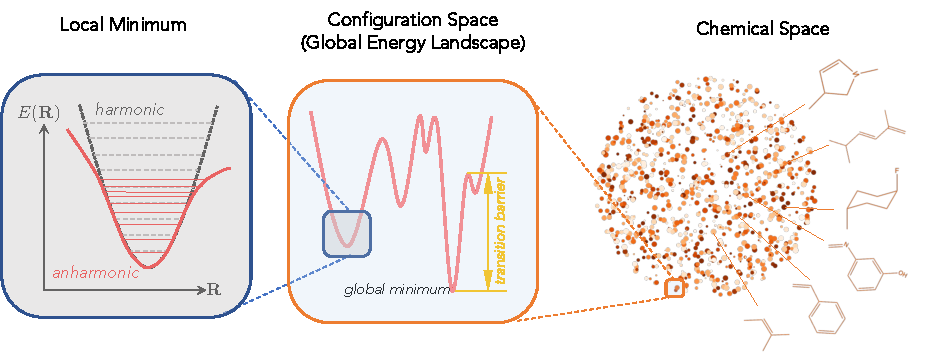
\includegraphics[width=\textwidth]{energy_landscapes_hierachical.pdf}
    \caption{Hierarchical view of the energy landscapes. (Left) Local minimum for a stable structure that is represented by an anharmonic potential well. The shape of the well close to its bottom can generally be well approximated by a harmonic potential (see \cref{sect:phonon} for detailed discussions). The topology of the potential well determines the vibrational behavior of the material, in which the dashed and solid horizontal lines represent the vibrational eigenenergy levels for the harmonic and anharmonic potential, respectively. (Middle) The configuration space for materials with a given chemical composition [or also known as the global energy landscape as for the cases of (a), (b) and (d) shown in \cref{fig:energy_landscape_examples}], which consists of multiple local minima that are separated by transition barriers for a structure to inter--convert between two different local minima. The global minimum corresponds to the structure with the lowest energy on the entire potential energy surface. This energy landscape belongs to a specific compound that is part of the larger (Right) chemical space, in which here a schematic illustration for the chemical space representing small organic molecules is shown. }
    \label{fig:energy_landscapes_hierachical}
\end{figure*}


For material scientists, the concept of PES is most widely known as the \textit{phase diagram}. It provides the information on the compositions and structures that are stable under a specific thermodynamic condition (\emph{e.g.} temperatures and pressures) for a given combination of elements, such as the Fe--C\cite{okamoto1992c} system that is critical in the steel--making industry and  Ti--O\cite{wahlbeck1966reinvestigation} [\cref{fig:energy_landscape_examples}(f)] system that has attracted enormous attention in guiding the development of photocatalysts. A particular compound may also possess multiple different phases each with a different physical property. The ABO$_3$ perovskite is a particularly interesting system with a rich phase behaviour. For instances, as temperature drops, \ce{BaTiO3} and \ce{KNbO3} undergo a sequence of phase transformations from cubic paraelectric, to tetragonal, orthorhombic, and finally the ferroelectric rhombohedral  phase, whereas \ce{PbTiO3} will only undergo cubic to ferroelectric tetragonal phase.\cite{ravel1998local} These phase transformation behaviours are strongly affected by the presence of the imaginary phonon modes\cite{fleury1968soft,pallikara2022physical} in the system, which is fundamentally dictated by the topology of the local minimum on the PES. This has also a strong implication in, for example, the behaviours of ion diffusions in solid--state batteries and electrolytes.\cite{he2017origin,di2019superionic} Phases that are non--stable under a given thermodynamic condition are generally referred to as the `metastable' phases\cite{aykol2018thermodynamic,sun2016thermodynamic} (similar to the case of high energy polymorphs for organic crystals described above). These phases may be of interesting physical properties, attracting interests to explore strategies to stabilize them under standard thermodynamic conditions, for instances, through the applications of chemical\cite{eitel2002preparation,protesescu2015nanocrystals,tan2017chemical} or mechanical  pressure. The presence of foreign dopants as well as the native defects in the material can also perturb the chemical bonding states in the material, hence changing the total system energy. As such, investigating the defect formation energy and/or chemical doping limits in materials comprise a large discipline of `defect chemistry' that is particularly important to guide the synthesis of materials with targeted properties.\cite{freysoldt2014first,anand2022convergent,norby2004hydrogen,robertson2011limits,lany2007dopability} Last but not least, the ability for high--entropy metal\cite{george2019high} or ceramic\cite{oses2020high}
alloys, which contains at least five different principal metal elements intermixed at a type of lattice site to form a homogeneous solid solution, is dictated by the competitions between the materials' enthalpy (bonding strengths) and configurational entropy, whereby the latter measures whether a specific spatial arrangements of atoms is energetically more preferred or degenerate compared to many other possible arrangements [\cref{fig:energy_landscape_examples}(e)].


Regardless of the different application scenarios discussed above, the concept of the PES can be  mathematically abstracted as a function $E(\bm{R})$ that maps the total energy of the system $E$ to the positions of $N$ atoms in the high--dimensional space $\bm{R}\in \mathbb{R}^{3N}$.  This generally defines a \emph{configuration space} in which both the types and numbers of different chemical elements in the material system, which will be denoted as $\mathcal{C}=\{\mathcal{X}_i,n_{i}\}$ (with $\mathcal{X}_i$ denotes the $i$--th chemical element in the compound and $n_i$ being its stoichiometry with $\sum_i n_i=N$), are fixed. Isomers of an organic compounds, different conformers of an organic molecule, high--entropy alloys with a fixed chemical composition, as well as different phases of perovskite \ce{BaTiO3}, can be characterised by the PES $E(\bm{R})$, where the experimentally observed structure corresponds to one of the many local minima on the PES. One can extend this to a collection of PES with different chemical compositions as $\left\{E_\chi(\bm{R})\vert \chi\in  \left\{\mathcal{C}_1,\mathcal{C}_2,\ldots\mathcal{C}_{k} \right\} \right\}$. This essentially defines a \emph{chemical space}, which is particularly popular in organic chemistry for searching drug--like and other functional compounds,\cite{reymond2015chemical,gomez2018automatic} whereas the phase diagram that is commonly used by material scientists can be considered as a restricted chemical space with fixed $\{\mathcal{X}_i\}$ but variable $\{n_i\}$.  As such, one can start to appreciate PES as a key universal concept in fundamental science, and  \cref{fig:energy_landscapes_hierachical} provides an overview behind this critical concept. 
